\documentclass[xcolor=dvipsnames,10pt]{beamer}
% ********** Styl prezentacji **********
%\usepackage{enumitem}
\usepackage{multirow}
\usepackage{tikz}
\usepackage{algorithm,algorithmic}
\usepackage{fancyvrb}
\usepackage{xcolor}
\usepackage{textcomp}
%\setdescription{style=multiline,topsep=10pt,leftmargin=5cm,font=\normalfont}
%\setdescription{style=multiline,leftmargin=1cm}
\mode<presentation>
{
\usetheme{Warsaw}
%\usetheme{default}
}
\author{Dr. Naeem Odat}
\institute[]{\includegraphics[width=1cm]{figures/ttulogo}\\College of Engineering\\Department of Communication and Computer Engineering}
\subject{Web Development and Programming}
\AtBeginSubsection[]
{
\begin{frame}<beamer>
\frametitle{Introduction}
\tableofcontents[currentsection,currentsubsection]
\end{frame}
}
\title[Interactivity with JavaScript]{Web Development and Programming\footnote{Michael Mendez. {\it The Missing Link: An Introduction to Web Development and Programming}. Open SUNY Textbooks 2014.}}
\subtitle{0107571\\Interactivity with JavaScript (AJAX and JSON)}
\date{}
\begin{document}
\begin{frame}
	
\titlepage

\end{frame}
\begin{frame}[fragile]
\frametitle{JavaScript}
\begin{block}{Introduction to Ajax}
\begin{itemize}
	\item AJAX = {\bf A}synchronous {\bf J}avaScript {\bf A}nd {\bf X}ML.
	\item AJAX is not a programming language.
	\item AJAX just uses a combination of:
\begin{itemize}
	\item A browser built-in XMLHttpRequest object (to request data from a web server)
	\item JavaScript and HTML DOM (to display or use the data)
\end{itemize}
\end{itemize}
\end{block}
\end{frame}
\begin{frame}[fragile]
\frametitle{JavaScript}
\begin{block}{How Ajax works}
\begin{center}
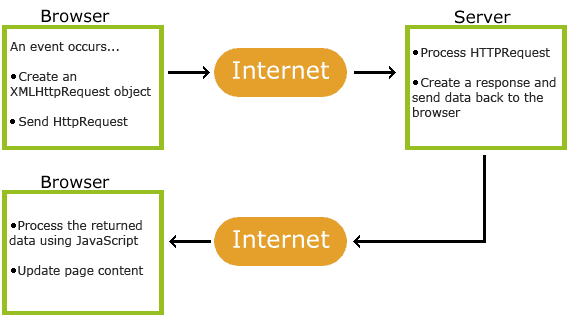
\includegraphics[width=\linewidth]{figures/ajax}
\end{center}
\end{block}
\end{frame}
\begin{frame}[fragile]
\frametitle{JavaScript}
\begin{block}{How Ajax works}
\begin{enumerate}
	\item An event occurs in a web page (the page is loaded, a button is clicked)
	\item An XMLHttpRequest object is created by JavaScript
	\item The XMLHttpRequest object sends a request to a web server
	\item The server processes the request
	\item The server sends a response back to the web page
	\item The response is read by JavaScript
	\item Proper action (like page update) is performed by JavaScript
\end{enumerate}	
\end{block}
\begin{block}{Demo}
	ajax.html
\end{block}
\end{frame}
\begin{frame}[fragile]
\frametitle{JavaScript}
\begin{block}{Quiz}
\begin{enumerate}
	\item One of the differences between a GET request and POST is that a GET request passes query parameters as part of the URL whereas POST request passes them as part of the body of the request.
	\begin{itemize}
		\item True
		\item False
	\end{itemize}
	\item Given the following JavaScript code snippet:
	\small
	{\color{blue}
	\begin{verbatim}
	var name = "";
	// Making an Ajax call here, i.e., sendGetRequest
	$ajaxUtils.sendGetRequest("someURL", function (request) {
	    name = "TTU";
	});	
	document.querySelector("#content").innerHTML = name;
	\end{verbatim}}
	\normalsize
	What will be the contents of the element with the 'id' value of 'content' after the execution of this JavaScript code?
	\begin{itemize}
		\item It will be empty
		\item TTU
		\item Whatever the server returns plus the word TTU
	\end{itemize}
\end{enumerate}
\end{block}
\end{frame}
\begin{frame}[fragile]
\frametitle{JavaScript}
\begin{block}{JSON}
\begin{itemize}
	\item Stands for: {\color{red}{\bf J}ava{\bf S}cript {\bf O}bject {\bf N}otation}
	\item Lightweight data-interchange format.
	\item Easy for humans to read and write.
	\item Easy for machines to parse and generate.
\end{itemize}
\end{block}
\end{frame}
\begin{frame}[fragile]
\frametitle{JavaScript}
\begin{block}{JSON Syntax Rules}
\begin{itemize}
	\item Subset of JavaScript object literals but:
	\begin{itemize}
		\item Property names must be in double quotes.
		\item String values must be in double quotes.
	\end{itemize}
\end{itemize}			
\end{block}
\begin{block}{Example}
\begin{verbatim}
{
    "firstName": "Naeem",
    "lastName": "Odat",
    "taughtCourse": 2
}
\end{verbatim}
\end{block}
\end{frame}
\begin{frame}[fragile]
\frametitle{JavaScript}
\begin{block}{Conversion between JSON string and JavaScript object}
\begin{itemize}
	\item To convert from JSON string to object:\\
	{\color{red}var obj=JSON.parse(jsonString);}
	\item To convert from JavaScript object to JSON string:\\
	{\color{red}var str=JSON.stringify(obj);}
\end{itemize}
\end{block}
\begin{block}{Demo}
json.html
\end{block}
\end{frame}
\begin{frame}[fragile]
\frametitle{JavaScript}
\begin{block}{Quiz}
\begin{enumerate}
	\item Another name for Object Literal is JSON.
	\begin{itemize}
		\item True
		\item False
	\end{itemize}	
	\item Identify invalid JSON string below:
\footnotesize
{\color{blue}		
\begin{verbatim}
'{
    "courseName": "InternetProgramming",
    "numberOfStudents": 6
}'
\end{verbatim}}
\begin{verbatim}
'{
    "courseName": "InternetProgramming",
    "studentsLoveCourse": true
}'
\end{verbatim}
{\color{blue}
\begin{verbatim}
'{
    'courseName': "InternetProgramming",
    'numberOfStudents': 6
}'
\end{verbatim}}
\begin{verbatim}
'{
    "courseName": {"name": "InternetProgramming"},
    "numberOfStudents": 6
}'
\end{verbatim}
\normalsize	
\end{enumerate}
\end{block}
\end{frame}
\begin{frame}[fragile]
\frametitle{JavaScript}
\begin{block}{Dynamic loading of a webpage}
\begin{itemize}
	\item Using Ajax a template of the webpage content is requested from the server.
	\item The data (in JSON format) that should be filled in the template is requested from the server.
	\item An appropriate JavaScript code will work on both to put each item in its place.
\end{itemize}	
\end{block}
\begin{block}{Demo}
	dynamicloading.html
\end{block}
\end{frame}














%\begin{frame}[fragile]
%\frametitle{JavaScript}
%\begin{block}{Output}	
%JavaScript doesn't have print or echo function, instead data is displayed by:
%\begin{itemize}
%	\item An alert box. (window.alert("Hello world");)
%	\item A prompt. (window.prompt"'Enter your name:");)
%	\item HTML output. (document.write("Hello world");)
%	\item HTML element. (element.innerHTML="Something";)
%	\item A browser console. (console.log("msg");)
%\end{itemize} 
%\end{block}
%\end{frame}
%\begin{frame}[fragile]
%\frametitle{JavaScript}
%\begin{block}{Operators and expressions}
%\begin{itemize}
%	\item Assignment operator (=). (var x=7;)
%	\item Arithmetic operators (+, -, *, /, \%, ++, --, +=).
%	\item String concatenation (+). (var str="My "+"Favorite";)
%	\item Boolean operators (==, !=, $>$, $<$, $>=$, $<=$). Returns false or true. (x=5; x==5;(return true) x!=5; (false)).
%	\item Boolean operators (===, !==). (Comparison of value and type.) \\
%	\begin{verbatim}
%	var x=12;
%	x=="12"; return true
%	x==="12"; return false
%	x!=="12"; return true
%	\end{verbatim}
%	\item Logical operators: \&\& (and), || (or), ! (not). Return true or false.
%\end{itemize}
%\end{block}
%\end{frame}
%\begin{frame}[fragile]
%\frametitle{JavaScript}
%\begin{block}{Functions}
%\begin{itemize}
%	\item Function syntax:
%	\includegraphics[width=\linewidth]{figures/functionsyntax}
%	\item Examples:
%	\begin{itemize}
%		\item \includegraphics[width=\linewidth]{figures/callfunction}
%		\item \includegraphics[width=\linewidth]{figures/functionreturn}
%	\end{itemize}	
%\end{itemize}
%\end{block}
%\end{frame}
%\begin{frame}[fragile]
%\frametitle{JavaScript}
%\begin{block}{Events}
%\begin{itemize}
%\item JavaScript API lets us add dynamic function calls based on special events.
%\item Events:
%\begin{itemize}
%	\item onclick. User clicks on an HTML element.
%	\item onmouseover. User moves the mouse over an HTML element.
%	\item onresize. Browser window is resized.
%	\item onload. Browser finishes loading the page. 
%\end{itemize} 
%\end{itemize}
%\end{block}
%\begin{block}{Example}
%\includegraphics[width=\linewidth]{figures/eventexample}
%\end{block}
%\end{frame}
%\begin{frame}[fragile]
%\frametitle{JavaScript}
%\begin{block}{this}
%	llll
%\end{block}
%\end{frame}
%\begin{frame}[fragile]
%\frametitle{JavaScript}
%\begin{block}{Arrays}
%In an array you can store multiple related pieces of information.
%\begin{itemize}
%	\item Declare an array: 
%	$var\ grades=[60,77,68,90,95,85];$
%	\item Get an array from DOM:
%	$var\ images=getElementsByClassName('imgs');$\\
%	$var\ itemLists=getElementsByTagName('li');$
%	
%\end{itemize}
%\end{block}
%\end{frame}
%\begin{frame}[fragile]
%\frametitle{JavaScript}
%\begin{block}{Arrays}
%	\begin{itemize}
%		\item Array can have elements of different types.\\
%		$var\ info=['Odat', 1123, "hello"];$
%		\item JavaScript arrays are objects:
%		\begin{itemize}
%			\item Can get its length. $info.length;$
%			\item Can be sorted. $info.sort();$
%			\item Elements can be appended into it. $info.push(x);$, $info[info.lemgth]=x;$
%			\item Can overwrite any element. $info[2]=x;$
%		\end{itemize} 
%	\end{itemize}
%\end{block}
%\end{frame}
%\begin{frame}[fragile]
%\frametitle{JavaScript}
%\begin{block}{For loops}
%\begin{verbatim}
%for(j=0;j<info.length;j++){
%    info[j]=j+1;
%}
%\end{verbatim}
%\end{block}
%\end{frame}
%\begin{frame}[fragile]
%\frametitle{JavaScript}
%\begin{block}{If statement}
%\begin{verbatim}
%if(condition){
%   //some statements
%}
%else{
%    //other statements
%}
%\end{verbatim}
%\end{block}
%\end{frame}
%\begin{frame}[fragile]
%\frametitle{JavaScript}
%\begin{block}{Forms}
%\begin{itemize}
%	\item Forms drive the internet.
%	\item Validation should be performed using JavaScript on the client-side, but validation would still have to be repeated on the server (JavaScript might be disabled).
%\begin{itemize}
%	\item Forms define places on a page where the user’s interaction can add, change, interact with, or remove the data in your system.
%	\item Form elements range from username and password style boxes to large text fields, drop down lists, checkboxes and more.
%	\item To create a form section.
%	\begin{verbatim}
%	<form name="" id="" action="" method=""></form>
%	\end{verbatim}
%\end{itemize}
%\end{itemize}
%\end{block}
%\end{frame}
%\begin{frame}[fragile]
%\frametitle{JavaScript}
%\begin{block}{HTML Form tag}
%Form tag contains one or more of the following elements:	
%\begin{itemize}
%	\item \textcolor{red}{$<legend>$}: To add title to the form.
%	\item \textcolor{red}{$<label>$}: Defines a label for a $<button>$, $<input>$, $<meter>$, $<output>$, $<progress>$, $<select>$, or $<textarea>$ element.
%	\item \textcolor{red}{$<input>$}: Specifies an input field where the user can enter data.
%	\item \textcolor{red}{$<textarea>$}: Defines a multi-line text input control.
%	\item \textcolor{red}{$<button>$}: Defines a clickable button.
%	\item \textcolor{red}{$<select>$}: Creates a drop-down list.
%	\item \textcolor{red}{$<option>$}: Defines an option in a select list.
%	\item \textcolor{red}{$<optgroup>$}: Groups related options in a drop-down list.
%	\item \textcolor{red}{$<fieldset>$}: Groups related elements in a form and draws a box around them.
%	\item \textcolor{red}{$<output>$}: Represents the result of a calculation.
%\end{itemize}
%\end{block}
%\end{frame}
%\begin{frame}[fragile]
%\frametitle{JavaScript}
%\begin{block}{HTML Form - input element}
%Input types:
%\begin{itemize}
%	\item text
%	\item email
%	\item password
%	\item radio
%	\item button
%	\item checkbox
%	\item submit
%	\item number
%	\item range
%	\item color
%	\item date
%	\item url
%\end{itemize}
%\end{block}
%\end{frame}
%\begin{frame}[fragile]
%\frametitle{JavaScript}
%\begin{block}{Validation}
%What to validate?	
%\begin{itemize}
%	\item The type of the input.
%	\item The format.
%	\item The value.
%\end{itemize}
%\end{block}
%\end{frame}
%\begin{frame}[fragile]
%\frametitle{JavaScript}
%\begin{block}{Validation}
%How to validate?	
%\begin{itemize}
%	\item Use new HTML5 input types (email, number, url)
%	\item Use HTML5 attributes (required, placeholder, min, max)
%	\item Use JavaScript functions (Write custom code to validate)
%\end{itemize}
%\end{block}
%\end{frame}
\end{document}

